\documentclass[aspectratio=169,t,11pt,table]{beamer}
\usepackage{slides,math}
\usepackage{subcaption}
\usepackage{graphicx}
\usepackage{xcolor}
\usepackage{varwidth}

% Define colors
\definecolor{accent}{HTML}{006896}
\definecolor{accent2}{HTML}{940034}

\title{\Large{\textbf{\navy{The Decline of Branch Banking}}}}
\author{\textbf{Rajesh Narayanan (LSU)}\\ 
\textbf{Dimuthu Ratnadiwakara (FRB-Richmond)*\\
\textbf{Philip Strahan (BC)}} } 
\date{Community Banking Research Conference  \hspace{0.2cm}|\hspace{0.2cm}October, 2025\\

\vspace{1.5cm}
\footnotesize{Disclaimer: The results and views are those of the authors and do not reflect those of the Federal Reserve Bank of Richmond, or the Federal Reserve System.}}


% Add bibliography references
\bibliography{resources/branchclosure}
\addbibresource{branchclosure.bib}


%\usepackage{xr}
%\externaldocument{_tables_figures_March2025.tex}

\begin{document}


% Title slide
\begin{frame}[noframenumbering,plain]
\maketitle
\end{frame}


\begin{frame}[c]{Research Question}
   What is driving branch openings and closings?
   
  \pause
   
  \begin{block}{Significance}
     Important to understanding ongoing industry restructuring 
     
     
  \end{block}
   
\end{frame}

\begin{frame}{We are Witnessing Massive and Rapid Debranching}
    \begin{center}
     \includegraphics[width=0.75\textwidth] {resources/figures/old/bank_branch_line_plot.jpg}   
    \end{center}
\end{frame}

\begin{frame}{Branch Closings Outpace Openings (by 3x)!}
    \begin{center}
     \includegraphics[width=0.75\textwidth]{resources/figures/JF figures/gross_open_closed.jpg}   
    \end{center}
\end{frame}

\begin{frame}{....Across Bank Size }
\centering
\vspace{1.5cm}

    \begin{varwidth}{\textwidth}
        \begin{figure}
            \includegraphics[height=0.45\textheight]{resources/figures/JF figures/closed_pct_by_size.jpg}
            
        \end{figure}
    \end{varwidth}
    \hfill
    \begin{varwidth}{\textwidth}
        \begin{figure}
            \includegraphics[height=0.45\textheight]{resources/figures/JF figures/open_pct_by_size.jpg}
         
        \end{figure}
    \end{varwidth}
\end{frame} 

\begin{frame}{Technology is Driving Debranching}

  
 Customer adoption of technology (e.g. Internet and Mobile banking) driving transition away from branches 
 \vspace{0.5cm}
 
            \begin{itemize}
                \item Financially sophisticated customers are interest rate sensitive
                \begin{itemize}
                    \item making it costly to retain deposits 
                    \item lowers deposit franchise value (the profits that can be earned from the stock of deposits from below-market pricing)
                \end{itemize}
                \vspace{0.5cm}
                \item Tech savvy customers place lower value on branch proximity
               
            \end{itemize}

\end{frame}

\begin{frame}[c]{Banks Close}

 
    
        \begin{itemize}
            \item Branches that have "costly" deposits (low deposit franchise value)
                \begin{itemize}
                    \item where the stock of deposits is low, and
                    \item depositors are rate-sensitive
                    \begin{itemize}
                        \item A 1 $\sigma$ increase in deposit $\beta$ increases the probability of closing a branch by about 10\% of the unconditional mean closure rate (=4\%) 
                    \end{itemize}
                   
                \end{itemize}
            \vspace{0.5cm}
            \item Branch with customers who can increasingly be served digitally
                \begin{itemize}
                    \item branch has low amenity value to customers
                \end{itemize}
            \vspace{0.5cm}
             \item Credit business (local lending) has very little influence
         \end{itemize}
\end{frame}

\begin{frame}[c]{Banks Open}

    
        \begin{itemize}
            \item Branches in deposit rich markets, but where
            \vspace{0.5cm}
           \item Depositors are rate sensitive                \begin{itemize}
                    \item A 1$\sigma$ increase in deposit $\beta$ raises the probability of opening a branch by about 25\% of the unconditional mean opening rate (=0.42\%)
            \end{itemize}
                \vspace{0.5cm}
                
        \item Rate-sensitive markets are easier to enter and attract customers by offering higher rates!       
        \end{itemize}
\end{frame}

\begin{frame}{Regulatory Forces Shaped Industry Restructuring in the Past}
\framesubtitle{Why \textit{Were} Branches so Important (1980-2008)?}


    \begin{itemize}
        \item Branch location affected competition (regulatory restrictions limited local-market contestability)
        \item Branch presence affected cost of information collection
        \item Extent of branch networks affected capital mobility
        \item Local branch concentration affected monetary policy transmission
    \end{itemize}
\vspace{0.5cm}
When regulatory constraints on branching were loosened 
\vspace{0.5cm}

    \begin{itemize}
        \item more competiton; bank M\& A exploded 
        \item more extenisve branch networks
        \item cheaper credit; better credit allocation
    \end{itemize}
\end{frame}

\begin{frame}{Technology Driving Ongoing Industry Restructuring}
\framesubtitle{Technology Promises to Further Reduce Frictions}
    

    \begin{itemize}
        \item Branchless competition; Greater market contestability
        \item More and cheaper credit; better terms for depositors
        \item More capital mobility
        \item Changes in information environment - tech/data substitutes for relationships?
    \end{itemize}

\end{frame}

\begin{frame}{Wide Variation in Customer Demographics Related to Technology Usage Across Banks }
Panel: 2022-2023\\
   \begin{table}[]
    \centering
   
    \vspace{0.5cm}
 
    \resizebox{0.8\textwidth}{!}{
       \begin{tabular}{lrrrrrrrr}
  \hline

& \multicolumn{4}{c}{Large Banks (Obs = 27)} & \multicolumn{4}{c}{Small Banks (Obs = 4,296)} \\
\cmidrule(l){2-5} \cmidrule(l){6-9}
Variable & Mean & SD & P10 & P90 & Mean & SD & P10 & P90 \\ 
  \hline
Age & 37.73 & 3.25 & 34.21 & 41.66 & 40.72 & 4.31 & 35.56 & 45.71 \\ 
  College educated fraction & 0.57 & 0.15 & 0.41 & 0.80 & 0.29 & 0.14 & 0.16 & 0.49 \\ 
  Deposit-weighted Pop. density & 0.52 & 0.14 & 0.36 & 0.69 & 0.15 & 0.21 & 0.01 & 0.57 \\ 
  Deposit beta & 0.32 & 0.14 & 0.18 & 0.55 & 0.18 & 0.12 & 0.04 & 0.35 \\ 
  Family income (000) & 88.81 & 39.06 & 59.00 & 117.00 & 58.28 & 18.45 & 39.00 & 80.00 \\ 
  Frac. deposits in sophisticated zipcodes & 0.82 & 0.17 & 0.56 & 1.00 & 0.46 & 0.41 & 0.00 & 1.00 \\ 
  HHI & 0.23 & 0.12 & 0.13 & 0.29 & 0.24 & 0.13 & 0.11 & 0.40 \\ 
  Stock market participation frac & 0.32 & 0.12 & 0.19 & 0.45 & 0.20 & 0.08 & 0.10 & 0.29 \\ 
   \hline
\end{tabular}
        }
  

\end{table} 
\end{frame}

\begin{frame}{Conceptual Framework}
    Exploit wide variation in local demographics related to technology usage across bank markets 
    \begin{itemize}
         \item Local Demographics $\longrightarrow$ Changes in the branch-level rate-sensitivity (Deposit $\beta$)
    \item Local Demographics $\longrightarrow$ Changes in Usage of Branches (Usage)
    \vspace{0.5cm}
    \item  High $\beta$ and Low Branch Usage $\longrightarrow$  More Branch Closures?
     \item  High $\beta$ and High Potential Branch Usage $\longrightarrow$  More Branch Openings?
    \end{itemize}
\end{frame}

\begin{frame}{Empirical Approach}
    \begin{itemize}
        \item Using data from ACS, IRS, Call Reports, SOD, HMDA, CRA, CBP, Advan (Cell-phone geolocation)
        \vspace{0.5cm}
        \item Build branch-level measures of $\beta$ and Usage
            \begin{itemize}
                \item Estimate demographic drivers of \textbf{bank-level} $\beta$ (over three rate-hiking cycles from 2001-2023) and Usage (2019-2023)
                \item Impute \textbf{branch-level} $\beta$ and Usage using coefficients from bank-level model
                        
            \end{itemize}
       
            \vspace{0.5cm}
        \item Estimate branch-level closure/openings models 
            \begin{itemize}
                \item Shut down investment in technology by banks (supply-side effects) using within-bank estimation
                \item Include Deposits, $\beta$, Usage, local lending variables, and other controls
            \end{itemize}
    \end{itemize}
\end{frame}

\begin{comment}
    
\begin{frame}{Distinction}

    \begin{itemize}
        \item Supply side: Investment in technology reduces branches (\cite{haendler2022keeping, jiang2022bank, koont2023digital})
        \item Low interest rates: reduces deposit franchise values and increases branches closures (\cite{sarto2023secular, kumarjames2025lowinterest}

\vspace{1.0cm}
Our focus:
\vspace{0.5cm}
        \item  Demand side: customer adoption of technology

        \item  Gross effects: closings and openings

    \end{itemize}

    
\end{frame}



    
\begin{frame}{Details}
\framesubtitle{Step 1: Build Bank-level Deposit $\beta$}

Follow (\cite{dss2023}) and compute DF/dollar for bank \textit{i}:

\centering
\vspace{1.0cm}

    \nonumber  DF_i &=\only<1>{(1-\beta_i - \frac{c_i}{r^p})\times\left(1 - \frac{1}{(1+r^p)^{10}}\right)}
    \only<2>{(1-\textcolor{red}{\beta_i} - \textcolor{black}{\frac{c_i}{r^p})\times\left(1 - \frac{1}{(1+r^p)^{10}}\right)}}
    \only<3>{{(1-\beta_i} - \textcolor{red}{\frac{c_i}{r^p}})\times\left(1 - \frac{1}{(1+r^p)^{10}}\right)}
    \only<4>{(1-\beta_i - \frac{c_i}{r^p})\times \textcolor{red}{\left(1 - \frac{1}{(1+r^p)^{10}}\right)}}
 
\vspace{1.0cm}

\only<2>{\textcolor{red}{$\beta_i$} = \textcolor{black}{$\Delta r_i^d/ \Delta r^f$}
 \textcolor{blue}{$r_i^d$} is the interest expense per dollar of deposits; \textcolor{blue}{$r^f$} is the Fed Funds rate}    
\only<3>{\textcolor{red}{$c_i$} is the operating cost per dollar of deposits; \textcolor{red}{$r^p$} is the the long-term interest rate, which is assumed to be 2.5 \%}    
\only<4>{\textcolor{red}{PVAIF_{2.5\%, 10}}}   

\end{frame}



\begin{frame}{Details}
\framesubtitle{Step 1: Build Bank-level Deposit $\beta$}
\begin{itemize}
    \item  Focus on three rate up-cycles: 2004-2006; 2016-2019; 2022-2024
    \centering
    \includegraphics[width=0.75\textwidth]{resources/figures/JF figures/FedFundsRate.png}
  \end{itemize}
\end{frame}

\begin{frame}{Details}
\framesubtitle{Step 1: Build Bank-level Deposit $\beta$}
    Estimate cross-bank regressions:
    \begin{equation*}
        \beta_{i,t} = \sum \gamma_t^k D_{i,t}^k + \eta_t HHI_{i,t} +\text{Other controls}+\varepsilon_{i,t}
    \end{equation*}
\centering
    where, $D_{i,t}^k$ is the $k^{th}$ demographic variable
    
\end{frame}




\begin{frame}{Details}
\framesubtitle{Step 2: Impute Branch-level DF ($\beta$)}

       Build branch-based DF with:
            \begin{itemize}
                \item Coefficients from Step 1 (bank-level regressions)
                \item Using demographics measured in each branch's zipcode
            \end{itemize}

    \begin{block}
         
         DF varies within bank, across branch network (absorb bank-time FE)
    \end{block} 
   
\end{frame}



\begin{frame}{Three Rate-Hiking Cycles from 2001-2023}
\framesubtitle{Early (2004-2006); Mid (2016-2019); Late (2022-2023)}

   % \item  Focus on three rate up-cycles: 2004-2006; 2016-2019; 2022-2024
    \centering
    \includegraphics[width=0.75\textwidth]{resources/figures/JF figures/FedFundsRate.png}

\end{frame}
\end{comment}

\begin{frame}{Bank-level Deposit $\beta$}
    \begin{center}
     \includegraphics[width=0.75\textwidth] {resources/figures/beta_density_bank.jpg}   
    \end{center}
\end{frame}

\begin{frame}{Demographic Drivers of Bank-Level Deposit Beta}
\\[-1.8ex]
\begin{table}[]
    \centering
    \resizebox{0.5\textwidth}{!}{
\begin{tabular}{@{\extracolsep{5pt}}lcccccc} 
\\[-1.8ex]\hline 
\hline \\[-1.8ex] 
 & \multicolumn{6}{c}{Deposit Beta} \\ 
\cline{2-7} 
 & Early Cyc. & Mid Cyc. & Late Cyc. & Early Cyc. & Mid Cyc. & Late Cyc.\\ 
\\[-1.8ex] & (1) & (2) & (3) & (4) & (5) & (6)\\ 
\hline \\[-1.8ex] 
\rowcolor<1>{yellow}  College frac                               & 0.4026$^{***}$  & 0.3353$^{***}$  & 0.5624$^{***}$  &                 &                 &   \\   
                                              & (0.0725)        & (0.0600)        & (0.1044)        &                 &                 &   \\   
\rowcolor<1>{yellow}   Stock market frac                          & 0.0863          & 0.1987$^{**}$   & 0.1409          &                 &                 &   \\   
                                              & (0.1004)        & (0.0812)        & (0.1435)        &                 &                 &   \\   
\rowcolor<1>{yellow}   Frac of deposits in sophisticated zipcodes &                 &                 &                 & 0.0763$^{***}$  & 0.0659$^{***}$  & 0.1039$^{***}$\\   
                                              &                 &                 &                 & (0.0138)        & (0.0123)        & (0.0208)\\   
   Age Q1-Q2                                  & 0.0068          & -0.0002         & 0.0015          & 0.0028          & -0.0016         & -0.0031\\   
                                              & (0.0129)        & (0.0107)        & (0.0181)        & (0.0127)        & (0.0105)        & (0.0177)\\   
   Age Q2-Q3                                  & -0.0204         & -0.0038         & 0.0097          & -0.0234$^{*}$   & -0.0021         & 0.0064\\   
                                              & (0.0149)        & (0.0123)        & (0.0210)        & (0.0141)        & (0.0118)        & (0.0199)\\   
\rowcolor<1>{yellow}   Age $>$Q3                                    & -0.0070         & -0.0641$^{***}$ & -0.0817$^{***}$ & -0.0094         & -0.0556$^{***}$ & -0.0796$^{***}$\\   
                                              & (0.0184)        & (0.0171)        & (0.0292)        & (0.0173)        & (0.0163)        & (0.0278)\\   
\rowcolor<1>{yellow}   log(Income)                                & -0.1278$^{***}$ & -0.0926$^{***}$ & -0.1295$^{***}$ & -0.0832$^{***}$ & -0.0186         & -0.0436\\   
                                              & (0.0267)        & (0.0234)        & (0.0395)        & (0.0233)        & (0.0201)        & (0.0338)\\   
   County deposit HHI                         & -0.1294$^{***}$ & -0.0578$^{*}$   & -0.1440$^{***}$ & -0.1309$^{***}$ & -0.0493         & -0.1428$^{**}$\\   
                                              & (0.0371)        & (0.0326)        & (0.0554)        & (0.0370)        & (0.0328)        & (0.0556)\\   
   log(Assets)                                & 0.0059          & 0.0158$^{***}$  & 0.0614$^{***}$  & 0.0077$^{*}$    & 0.0179$^{***}$  & 0.0645$^{***}$\\   
                                              & (0.0043)        & (0.0033)        & (0.0053)        & (0.0043)        & (0.0033)        & (0.0053)\\   
   Population density                         & 0.0394          & 0.0921$^{***}$  & 0.2802$^{***}$  & 0.1364$^{***}$  & 0.1806$^{***}$  & 0.4203$^{***}$\\   
                                              & (0.0355)        & (0.0285)        & (0.0484)        & (0.0313)        & (0.0248)        & (0.0422)\\   
   Transaction Accounts/Assets                & -0.5629$^{***}$ & -0.3281$^{***}$ & -0.2854$^{***}$ & -0.5650$^{***}$ & -0.3274$^{***}$ & -0.2935$^{***}$\\   
                                              & (0.0720)        & (0.0484)        & (0.0677)        & (0.0721)        & (0.0486)        & (0.0678)\\   
   Uninsured Deposits/Deposits                & 0.7734$^{***}$  & -0.0529$^{*}$   & 0.3780$^{***}$  & 0.8114$^{***}$  & -0.0253         & 0.4153$^{***}$\\   
                                              & (0.0364)        & (0.0299)        & (0.0512)        & (0.0356)        & (0.0298)        & (0.0511)\\   
  Constant                                   & 1.773$^{***}$   & 1.175$^{***}$   & 1.059$^{**}$    & 1.336$^{***}$   & 0.4230$^{*}$    & 0.1917\\   
  & (0.2844)        & (0.2505)        & (0.4218)        & (0.2546)        & (0.2190)        & (0.3681)\\   
    \\
   Observations                               & 5,539           & 4,906           & 4,405           & 5,539           & 4,906           & 4,405\\  
   R$^2$                                      & 0.17833         & 0.09642         & 0.20750         & 0.17544         & 0.08855         & 0.20282\\  
   % Adjusted R$^2$                             & 0.17670         & 0.09439         & 0.20551         & 0.17395         & 0.08669         & 0.20101\\ 
\hline 
\hline \\[-1.8ex] 
\textit{Note:}  & \multicolumn{6}{r}{$^{*}$p$<$0.1; $^{**}$p$<$0.05; $^{***}$p$<$0.01} \\ 
\end{tabular} 
    }
   
\end{table}
\end{frame}


\begin{frame}{Branch-level Deposit $\beta$}

    \begin{center}
     \includegraphics[width=0.75\textwidth] {resources/figures/beta_density_branch.jpg}   
    \end{center}
\end{frame}

 
\begin{frame}{Branch-level Deposit $\beta$}
\framesubtitle{Early vs. Mid Cycle Correlation}
    \begin{center}
     \includegraphics[width=0.60\textwidth] {resources/figures/df_scatter_branch_early_mid.jpg}   
    \end{center}
\end{frame}



\begin{frame}{Branch-level Deposit $\beta$}
\framesubtitle{Mid vs. Late Cycle Correlation}
    \begin{center}
     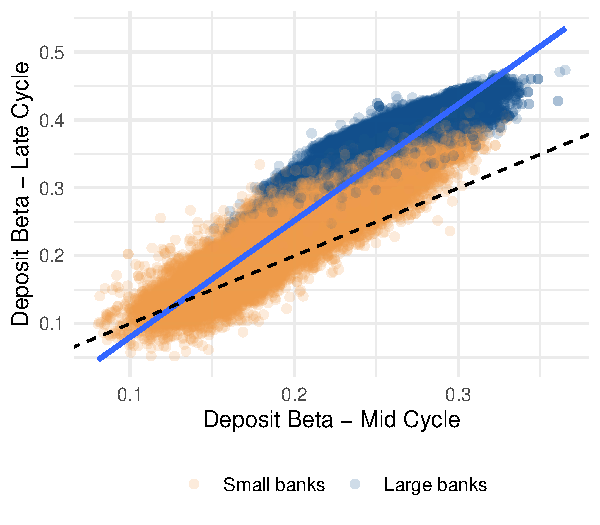
\includegraphics[width=0.60\textwidth] {resources/figures/df_scatter_branch_mid_late.jpg}   
    \end{center}
\end{frame}

\begin{frame}{Demographic Drivers of Branch Usage}
\\[-1.8ex]
    \begin{table}[]
    \centering
    \resizebox{0.5\textwidth}{!}{
\begin{tabular}{@{\extracolsep{5pt}}lcccc} 
\\[-1.8ex]\hline 
\hline \\[-1.8ex] 
%  & \multicolumn{4}{c}{\textit{Dependent variable:}} \\ 
% \cline{2-5} 
 & \multicolumn{2}{c}{Drop in visits} & \multicolumn{2}{c}{log(distance km)} \\ 
 \\[-1.8ex] & Large banks & Small banks & Large banks & Small banks\\ 
\\[-1.8ex] & (1) & (2) & (3) & (4)\\ 
\hline \\[-1.8ex] 
\rowcolor<1>{yellow}    Sophisticated zipcode & 0.0652$^{***}$  & 0.1034$^{***}$  & 0.1841$^{***}$  & 0.1212$^{***}$\\   
                         & (0.0099)        & (0.0077)        & (0.0187)        & (0.0092)\\   
\rowcolor<1>{yellow}   Age Q1-Q2             & -0.0200$^{***}$ & -0.0410$^{***}$ & -0.0661$^{***}$ & -0.0440$^{***}$\\   
                         & (0.0043)        & (0.0080)        & (0.0122)        & (0.0099)\\   
\rowcolor<1>{yellow}   Age Q2-Q3             & -0.0703$^{***}$ & -0.1039$^{***}$ & -0.0795$^{***}$ & -0.0515$^{***}$\\   
                         & (0.0076)        & (0.0094)        & (0.0204)        & (0.0127)\\   
   Age $>$Q3               & -0.0710$^{***}$ & -0.1264$^{***}$ & 0.0280          & 0.0888$^{***}$\\   
                         & (0.0113)        & (0.0124)        & (0.0247)        & (0.0168)\\   
\rowcolor<1>{yellow}   log(Income)           & 0.0053          & 0.0093$^{**}$   & -0.0698$^{***}$ & -0.0354$^{***}$\\   
                         & (0.0042)        & (0.0043)        & (0.0084)        & (0.0051)\\   
   log(Deposits)         & 0.0185$^{***}$  & 0.0278$^{***}$  & 0.0291$^{**}$   & -0.0129$^{**}$\\   
                         & (0.0064)        & (0.0040)        & (0.0115)        & (0.0057)\\   
   Population density    & 0.3688$^{***}$  & 0.5439$^{***}$  & -0.3718$^{***}$ & -0.1433$^{**}$\\   
                         & (0.0405)        & (0.0248)        & (0.0282)        & (0.0556)\\ 
       \hline
   Bank FE   & $\checkmark$    & $\checkmark$    & $\checkmark$    & $\checkmark$\\   
   State FE  & $\checkmark$    & $\checkmark$    & $\checkmark$    & $\checkmark$\\  \hline
  Observations          & 26,521          & 26,276          & 26,560          & 26,355\\  
   R$^2$                 & 0.26680         & 0.43095         & 0.19958         & 0.33392\\  
   %Within R$^2$             & 0.08109         & 0.08541         & 0.06157         & 0.01908\\  
\hline 
\hline \\[-1.8ex] 
\textit{Note:}  & \multicolumn{4}{r}{$^{*}$p$<$0.1; $^{**}$p$<$0.05; $^{***}$p$<$0.01} \\ 
\end{tabular} 
}

\end{table}
\end{frame}

\begin{frame}{Deposit $\beta$ and Branch Closure}
    \begin{figure}
    \centering
    
    \includegraphics[width=0.75\textwidth]{resources/figures/univar_branch.pdf}
   
\end{figure}
\end{frame}

\begin{frame}{Predicting Branch Closures}
\\[-1.8ex]
    \begin{table}[]
    \centering
   
    \resizebox{0.5\textwidth}{!}{
\begin{tabular}{@{\extracolsep{5pt}}lcccccc} 
\\[-1.8ex]\hline 
\hline \\[-1.8ex] 
 & \multicolumn{6}{c}{Closed=1} \\ 
\cline{2-7} 
 & \multicolumn{2}{c}{Full sample} & \multicolumn{2}{c}{Large banks} & \multicolumn{2}{c}{Small banks} \\ 
% \\[-1.8ex] & (1) & (2) & (3) & (4) & (5) & (6)\\ 
% \hline \\[-1.8ex] 
                                    & (1)                    & (2)             & (3)             & (4)             & (5)             & (6)\\  
   \midrule 
\rowcolor<1>{yellow}   Deposit Beta                     & 0.1286$^{***}$         & 0.1700$^{***}$  & 0.1719$^{***}$  & 0.2586$^{***}$  & 0.1007$^{***}$  & 0.0966$^{***}$\\   
                                    & (0.0145)               & (0.0213)        & (0.0232)        & (0.0282)        & (0.0127)        & (0.0140)\\   
\rowcolor<2>{yellow}   log(Deposits)                    & -0.0199$^{***}$        & -0.0200$^{***}$ & -0.0231$^{***}$ & -0.0232$^{***}$ & -0.0175$^{***}$ & -0.0175$^{***}$\\   
                                    & (0.0006)               & (0.0007)        & (0.0010)        & (0.0011)        & (0.0005)        & (0.0005)\\   
   Acq. branch/presence             & 0.0516$^{***}$         & 0.0494$^{***}$  & 0.0562$^{***}$  & 0.0512$^{***}$  & 0.0447$^{***}$  & 0.0428$^{***}$\\   
                                    & (0.0066)               & (0.0068)        & (0.0108)        & (0.0113)        & (0.0047)        & (0.0046)\\   
   Branch owned 3plus years         & -0.0055$^{***}$        & -0.0054$^{***}$ & -0.0057$^{*}$   & -0.0068$^{**}$  & -0.0064$^{***}$ & -0.0065$^{***}$\\   
                                    & (0.0015)               & (0.0014)        & (0.0030)        & (0.0029)        & (0.0011)        & (0.0011)\\   
   log(Bank-County Mortgage Volume) & -0.0003                & -0.0006$^{*}$   & -0.0009         & -0.0007         & -0.0001         & -0.0005$^{**}$\\   
                                    & (0.0003)               & (0.0003)        & (0.0008)        & (0.0015)        & (0.0002)        & (0.0002)\\   
   log(Bank-County CRA Volume)      & $-7.86e\text{-}5$  & -0.0003         & 0.0006          & 0.0009          & -0.0002         & -0.0004$^{*}$\\   
                                    & (0.0003)               & (0.0003)        & (0.0005)        & (0.0008)        & (0.0003)        & (0.0003)\\   
   Deposit 3yr growth               & 0.0016                 &                 & 0.0037$^{**}$   &                 & 0.0007          &   \\   
                                    & (0.0010)               &                 & (0.0018)        &                 & (0.0011)        &   \\   
\rowcolor<3>{yellow}   Mortgage 3yr growth              & -0.0071$^{**}$         &                 & -0.0075         &                 & -0.0052$^{**}$  &   \\   
                                    & (0.0028)               &                 & (0.0049)        &                 & (0.0026)        &   \\   
\rowcolor<3>{yellow}   CRA 3yr growth                   & -0.0012                &                 & -0.0004         &                 & -0.0013         &   \\   
                                    & (0.0008)               &                 & (0.0019)        &                 & (0.0008)        &   \\   
   Establishments 3yr growth        & -0.1332$^{***}$        &                 & -0.2509$^{***}$ &                 & -0.0265         &   \\   
                                    & (0.0258)               &                 & (0.0448)        &                 & (0.0180)        &   \\   
   Payroll 3yr growth               & -0.0002                &                 & -0.0057         &                 & 0.0053          &   \\   
                                    & (0.0056)               &                 & (0.0100)        &                 & (0.0065)        &   \\   
   Low to Moderate Income Area      & -0.0040$^{***}$        &                 & -0.0099$^{***}$ &                 & 0.0013          &   \\   
                                    & (0.0015)               &                 & (0.0024)        &                 & (0.0011)        &   \\   
    \\

   \hline
   State $\times$ Year FE     & $\checkmark$    &                 & $\checkmark$    &                 & $\checkmark$           & \\  
   Bank $\times$ Year FE      & $\checkmark$    & $\checkmark$    & $\checkmark$    & $\checkmark$    & $\checkmark$           & $\checkmark$\\   
   County $\times$ Year FE    &                 & $\checkmark$    &                 & $\checkmark$    &                        & $\checkmark$\\   
   \hline
   Observations                     & 1,592,669              & 1,592,669       & 690,038         & 690,038         & 902,631         & 902,631\\  
   R$^2$                            & 0.09844                & 0.13106         & 0.05019         & 0.11084         & 0.15682         & 0.21460\\  
   Mean Closure Rate                            & \multicolumn{2}{c}{0.025}        &  \multicolumn{2}{c}{0.031}        &  \multicolumn{2}{c}{0.021}\\  
   % Within R$^2$                     & 0.01668                & 0.01643         & 0.01770         & 0.01710         & 0.01623         & 0.01589\\

\hline 
\hline \\[-1.8ex] 
\textit{Note:}  & \multicolumn{6}{r}{$^{*}$p$<$0.1; $^{**}$p$<$0.05; $^{***}$p$<$0.01} \\ 
\end{tabular} 
    }
   
\end{table}
\end{frame}

\begin{frame}{Predicting Branch Closures (with Usage)}
\\[-1.8ex]
    \begin{table}[]
    \centering
    \resizebox{0.75\textwidth}{!}{
\begin{tabular}{@{\extracolsep{5pt}}lcccccccc} 
\\[-1.8ex]\hline 
\hline \\[-1.8ex] 
 & \multicolumn{8}{c}{Closed=1} \\ 
\cline{2-9} 
 & \multicolumn{4}{c}{Large banks} & \multicolumn{4}{c}{Small banks} \\ 
\\[-1.8ex] & (1) & (2) & (3) & (4) & (5) & (6) & (7) & (8)\\ 
\hline \\[-1.8ex] 
     Deposit Beta                    & 0.1793$^{***}$ & 0.2378$^{***}$ & 0.1053$^{***}$ & 0.1156$^{***}$ & 0.0827$^{***}$ & 0.0573$^{**}$ & 0.0583$^{***}$ & 0.0406\\   
                                   & (0.0277)       & (0.0379)       & (0.0264)       & (0.0388)       & (0.0227)       & (0.0291)      & (0.0222)       & (0.0288)\\  
     log(Deposits)                   & -0.0249$^{***}$ & -0.0247$^{***}$ & -0.0262$^{***}$ & -0.0263$^{***}$ & -0.0143$^{***}$ & -0.0140$^{***}$ & -0.0144$^{***}$ & -0.0142$^{***}$\\   
                                   & (0.0047)        & (0.0048)        & (0.0047)        & (0.0048)        & (0.0009)        & (0.0010)        & (0.0009)        & (0.0010)\\   
   Drop in visits                  &                &                & 0.0116         & 0.0143         &                &               & 0.0090$^{***}$ & 0.0055$^{***}$\\   
                                   &                &                & (0.0078)       & (0.0099)       &                &               & (0.0016)       & (0.0020)\\   
   log(Distance km)                &                &                & 0.0164$^{***}$ & 0.0205$^{***}$ &                &               & 0.0014         & 0.0040$^{**}$\\   
                                   &                &                & (0.0027)       & (0.0035)       &                &               & (0.0013)       & (0.0017)\\      \hline
   Controls                  & $\checkmark$   & $\checkmark$   & $\checkmark$    & $\checkmark$    & $\checkmark$   & $\checkmark$   & $\checkmark$    & $\checkmark$\\   
      State $\times$ Year FE   & $\checkmark$   &                & $\checkmark$    &                 &                &                & $\checkmark$    & \\  
   Bank $\times$ Year FE    & $\checkmark$   & $\checkmark$   & $\checkmark$    & $\checkmark$    & $\checkmark$   & $\checkmark$   & $\checkmark$    & $\checkmark$\\   
   County $\times$ Year FE  &                & $\checkmark$   &                 & $\checkmark$    & $\checkmark$   & $\checkmark$   &                 & $\checkmark$\\
   \hline 
  Observations                    & 58,459         & 58,459         & 58,432         & 58,432         & 73,003         & 73,003        & 72,825         & 72,825\\  
   R$^2$                           & 0.03228        & 0.09030        & 0.03382        & 0.09201        & 0.10932        & 0.16491       & 0.10988        & 0.16540\\  
    Mean Closure Rate                           &\multicolumn{4}{c}{0.040}&\multicolumn{4}{c}{0.017}\\  
%   Within R$^2$              & 0.01427        & 0.01378        & 0.01548         & 0.01538         & 0.01232        & 0.01232        & 0.01346         & 0.01258\\  

\hline 
\hline \\[-1.8ex] 
\textit{Note:}  & \multicolumn{8}{r}{$^{*}$p$<$0.1; $^{**}$p$<$0.05; $^{***}$p$<$0.01} \\ 
\end{tabular} 
        }
   
\end{table}
\end{frame}

\begin{frame}{Predicting Branch Openings}
\\[-1.8ex]
   \begin{table}[]
    \centering
    \resizebox{0.5\textwidth}{!}{
\begin{tabular}{@{\extracolsep{5pt}}lcccccc} 
\\[-1.8ex]\hline 
\hline \\[-1.8ex] 
 & \multicolumn{6}{c}{Opening=1} \\ 
\cline{2-7} 
 & \multicolumn{2}{c}{Full sample} & \multicolumn{2}{c}{Large banks} & \multicolumn{2}{c}{Small banks} \\ 
\\[-1.8ex] & (1) & (2) & (3) & (4) & (5) & (6)\\ 
\hline \\[-1.8ex] 
\rowcolor<1>{yellow}   Deposit Beta                          & 0.0204$^{***}$          & 0.0273$^{***}$         & 0.0441$^{***}$        & 0.0586$^{***}$ & 0.0172$^{***}$          & 0.0239$^{***}$\\   
                                         & (0.0017)                & (0.0016)               & (0.0108)              & (0.0108)       & (0.0009)                & (0.0011)\\   
\rowcolor<1>{yellow}   log(Zip code deposits)                & 0.0003$^{***}$          & 0.0003$^{***}$         & 0.0005$^{***}$        & 0.0006$^{***}$ & 0.0003$^{***}$          & 0.0003$^{***}$\\   
                                         & ($1.83e\text{-}5$)  & ($1.8e\text{-}5$)  & ($10e\text{-}5$)  & (0.0001)       & ($9.41e\text{-}6$)  & ($9.79e\text{-}6$)\\    
 log(County mortgage volume)    & -0.0002                 &                        & 0.0016$^{***}$        &                & -0.0009$^{***}$         &   \\   
                                         & (0.0002)                &                        & (0.0005)              &                & ($8.51e\text{-}5$)  &   \\   
   log(County CRA volume)         & 0.0004$^{**}$           &                        & -0.0006$^{*}$         &                & 0.0009$^{***}$          &   \\   
                                         & (0.0002)                &                        & (0.0003)              &                & ($7.22e\text{-}5$)  &   \\   
                                         
   Deposit 3yr growth                    & -0.0003$^{**}$          &                        & 0.0009                &                & -0.0005$^{***}$         &   \\   
                                         & (0.0001)                &                        & (0.0007)              &                & (0.0001)                &   \\   
   Mortgage 3yr growth                   & 0.0003                  &                        & -0.0059$^{**}$        &                & 0.0015$^{***}$          &   \\   
                                         & (0.0006)                &                        & (0.0025)              &                & (0.0003)                &   \\   
   CRA 3yr growth                        & -0.0004                 &                        & 0.0012                &                & -0.0008$^{***}$         &   \\   
                                         & (0.0002)                &                        & (0.0008)              &                & (0.0002)                &   \\   
     Establishments 3yr growth             & 0.0279$^{***}$          &                        & 0.0428$^{***}$        &                & 0.0238$^{***}$          &   \\   
                                         & (0.0023)                &                        & (0.0081)              &                & (0.0019)                &   \\   
   Payroll 3yr growth                    & 0.0017$^{**}$           &                        & 0.0046                &                & 0.0012                  &   \\   
                                         & (0.0007)                &                        & (0.0030)              &                & (0.0007)                &   \\   
   Low to Moderate Income Area           & -0.0007$^{***}$         &                        & 0.0004                &                & -0.0010$^{***}$         &   \\   
                                         & (0.0001)                &                        & (0.0006)              &                & (0.0001)                &   \\   
    \hline
       State $\times$ Year FE   & $\checkmark$            &                         & $\checkmark$            &                 & $\checkmark$            & \\  
   Bank $\times$ Year FE    & $\checkmark$            & $\checkmark$            & $\checkmark$            & $\checkmark$    & $\checkmark$            & $\checkmark$\\   
   County $\times$ Year FE  &                         & $\checkmark$            &                         & $\checkmark$    &                         & $\checkmark$\\  
   \hline
   Observations                          & 12,579,759              & 12,580,951             & 1,409,902             & 1,410,042      & 11,169,857              & 11,170,909\\  
   R$^2$                                 & 0.02837                 & 0.03894                & 0.01978               & 0.03866        & 0.03227                 & 0.04800\\  
    Mean Opening Rate                            & \multicolumn{2}{c}{0.0019}        &  \multicolumn{2}{c}{0.0039}        &  \multicolumn{2}{c}{ 0.0016}\\  
 
\hline 
\hline \\[-1.8ex] 
\textit{Note:}  & \multicolumn{6}{r}{$^{*}$p$<$0.1; $^{**}$p$<$0.05; $^{***}$p$<$0.01} \\ 
\end{tabular} 
    }
   
\end{table} 
\end{frame}

\begin{frame}{Predicting Branch Openings (with Usage)}
\\[-1.8ex]
    \begin{table}[]
    \centering
    \resizebox{0.75\textwidth}{!}{
\begin{tabular}{@{\extracolsep{5pt}}lcccccccc} 
\\[-1.8ex]\hline 
\hline \\[-1.8ex] 
 & \multicolumn{8}{c}{Opening=1} \\ 
\cline{2-9} 
 & \multicolumn{4}{c}{Large banks} & \multicolumn{4}{c}{Small banks} \\ 
\\[-1.8ex] & (1) & (2) & (3) & (4) & (5) & (6) & (7) & (8)\\ 
\hline \\[-1.8ex] 
  Deposit Beta                 & 0.0308$^{**}$         & 0.0275$^{**}$ & 0.0282$^{**}$         & 0.0261$^{*}$  & 0.0019         & 0.0042$^{***}$ & 0.0012                  & 0.0040$^{***}$\\   
                                & (0.0124)              & (0.0132)      & (0.0112)              & (0.0130)      & (0.0012)       & (0.0014)       & (0.0012)                & (0.0014)\\   

     log(Zip code deposits)      & 0.0019$^{**}$ & 0.0020$^{**}$ & 0.0018$^{**}$ & 0.0020$^{**}$ & 0.0006$^{***}$         & 0.0007$^{***}$          & 0.0006$^{***}$          & 0.0006$^{***}$\\   
                               & (0.0008)      & (0.0009)      & (0.0008)      & (0.0009)      & ($4.2e\text{-}5$)  & ($4.49e\text{-}5$)  & ($4.1e\text{-}5$)   & ($4.42e\text{-}5$)\\    
 
  
   Drop in visits               &                       &               & 0.0019                & 0.0018        &                &                & 0.0007$^{***}$          & 0.0008$^{***}$\\   
                                &                       &               & (0.0015)              & (0.0015)      &                &                & (0.0001)                & (0.0002)\\   
   log(Distance km)             &                       &               & 0.0004                & 0.0001        &                &                & $3.29e\text{-}5$    & $-8.77e\text{-}5$\\    
                                &                       &               & (0.0005)              & (0.0007)      &                &                & ($8.49e\text{-}5$)  & ($9.56e\text{-}5$)\\    
\hline
   Controls                    & $\checkmark$   & $\checkmark$  & $\checkmark$   & $\checkmark$          & $\checkmark$   & $\checkmark$    & $\checkmark$            & $\checkmark$\\   
     Bank $\times$ Year FE    & $\checkmark$   & $\checkmark$  & $\checkmark$   & $\checkmark$          & $\checkmark$   & $\checkmark$    & $\checkmark$            & $\checkmark$\\   
   State $\times$ Year FE   & $\checkmark$   &               & $\checkmark$   &                       & $\checkmark$   &                 & $\checkmark$            & \\  
   County $\times$ Year FE  &                & $\checkmark$  &                & $\checkmark$          &                & $\checkmark$    &                         & $\checkmark$\\ 
   \hline
   Observations                 & 112,960               & 112,960       & 112,540               & 112,540       & 711,861        & 711,861        & 710,463                 & 710,463\\  
   R$^2$                        & 0.01587               & 0.04090       & 0.01606               & 0.04110       & 0.03189        & 0.05181        & 0.03206                 & 0.05196\\
   Mean Opening Rate                           &\multicolumn{4}{c}{0.0035}&\multicolumn{4}{c}{0.0011}\\  %  Within R$^2$                & 0.00410        & 0.00250       & 0.00422        & 0.00256               & 0.00080        & 0.00079         & 0.00083                 & 0.00082\\  

\hline 
\hline \\[-1.8ex] 
\textit{Note:}  & \multicolumn{8}{r}{$^{*}$p$<$0.1; $^{**}$p$<$0.05; $^{***}$p$<$0.01} \\ 
\end{tabular} 
        }
    
\end{table}
\end{frame}

\begin{comment}
    

\begin{frame}{Details}
\framesubtitle{Step 3: Run Branch Opening and Closing Models}

    \begin{itemize}
        \item Estimate probability of branch openings \& closings based on:
            \begin{itemize}
                \item  Branch-level DF
                \item  Local (lagged) growth in Deposits, CRA loans, and Mortgages
                \item  Other economic controls (HHI, Population density, local real growth)
            \end{itemize}

        \item Candidates for closing
            \begin{itemize}
                \item Branches in existence at t-1
            \end{itemize}
            
        \item Candidate zip-codes for opening
            \begin{itemize}
                \item Zips in CBSAs where bank owned a branch at t-1
                \item Zips in CBSAs where bank opened a branch at t
                \item Drop all zips with no branches (ever)
            \end{itemize}
    \end{itemize}
\end{frame}

\begin{frame}{Predicting Closure}

\begin{table}[]
    \centering
   
    \resizebox{0.80\textwidth}{!}{
\begin{tabular}{@{\extracolsep{5pt}}lcccccc} 
\\[-1.8ex]\hline 
\hline \\[-1.8ex] 
 & \multicolumn{6}{c}{Closed=1} \\ 
\cline{2-7} 
 & \multicolumn{2}{c}{Full sample} & \multicolumn{2}{c}{Large banks} & \multicolumn{2}{c}{Small banks} \\ 
\\[-1.8ex] & (1) & (2) & (3) & (4) & (5) & (6)\\ 
\hline \\[-1.8ex] 
  DF per dollar               & \textbf{-0.5067$^{***}$} & \textbf{-0.7017$^{***}$} & \textbf{-0.6339$^{***}$} & \textbf{-0.9833$^{***}$} & \textbf{-0.4451$^{***}$}        & \textbf{-0.4498}$^{***}$\\   
                               
   log(Deposits)               & -0.0205$^{***}$ & -0.0206$^{***}$ & -0.0233$^{***}$ & -0.0233$^{***}$ & -0.0183$^{***}$        & -0.0183$^{***}$\\   
                              
   Acq. branch/presence        & 0.0531$^{***}$  & 0.0504$^{***}$  & 0.0568$^{***}$  & 0.0521$^{***}$  & 0.0477$^{***}$         & 0.0448$^{***}$\\   
                                 
   Branch owned 3plus years    & -0.0055$^{***}$ & -0.0059$^{***}$ & -0.0054$^{*}$   & -0.0061$^{*}$   & -0.0062$^{***}$        & -0.0067$^{***}$\\   
                            
   Deposit 3yr growth          & 0.0006          &                 & 0.0023          &                 & $-2.62e\text{-}5$  &   \\   
                              
   \textbf{Mortgage 3yr growth}         & -0.0071$^{**}$  &                 & -0.0077         &                 & -0.0054$^{*}$          &   \\   
                              
 \textbf{ CRA 3yr growth}              & -0.0018$^{**}$  &                 & -0.0013         &                 & -0.0017$^{*}$          &   \\   
                             
   Establishments 3yr growth   & -0.1440$^{***}$ &                 & -0.2644$^{***}$ &                 & -0.0376$^{**}$         &   \\   
                              
   Payroll 3yr growth          & 0.0002          &                 & -0.0072         &                 & 0.0067                 &   \\   
                              
   Low to Moderate Income Area & -0.0049$^{***}$ &                 & -0.0109$^{***}$ &                 & 0.0007                 &   \\   
                              
\hline
   State $\times$ Year FE     & $\checkmark$    &                 & $\checkmark$    &                 & $\checkmark$           & \\  
   Bank $\times$ Year FE      & $\checkmark$    & $\checkmark$    & $\checkmark$    & $\checkmark$    & $\checkmark$           & $\checkmark$\\   
   County $\times$ Year FE    &                 & $\checkmark$    &                 & $\checkmark$    &                        & $\checkmark$\\   
   \hline
   Observations                & 1,594,989       & 1,594,989       & 690,261         & 690,261         & 904,728                & 904,728\\  
   R$^2$                       & 0.09939         & 0.13228         & 0.05002         & 0.11053         & 0.15713                & 0.21608\\  
%   Within R$^2$                & 0.01713         & 0.01687         & 0.01789         & 0.01727         & 0.01691                & 0.01652\\  

\hline 
\hline \\[-1.8ex] 
\textit{Note:}  & \multicolumn{6}{r}{$^{*}$p$<$0.1; $^{**}$p$<$0.05; $^{***}$p$<$0.01} \\ 
\end{tabular} 
    }
   
\end{table}
\end{frame}

\begin{frame}{Predicting Closures Over Time}

\begin{table}[]
    \centering
    
    \vspace{0.25cm}

    \resizebox{0.8\textwidth}{!}{
\begin{tabular}{@{\extracolsep{5pt}}lcccccccc} 

 & \multicolumn{8}{c}{Closed=1} \\ 
\cline{2-9} 
 & \multicolumn{2}{c}{2001:2007} & \multicolumn{2}{c}{2008:2011} & \multicolumn{2}{c}{2012:2019} & \multicolumn{2}{c}{2020:2023} \\ 
\\[-1.8ex] & (1) & (2) & (3) & (4) & (5) & (6) & (7) & (8)\\ 
\hline \\[-1.8ex] 

{\small Panel A: Large Banks}\\
\hline \\[-1.8ex] 

    DF per dollar               & -0.7019$^{***}$ & -0.5859$^{***}$ & -0.7235$^{***}$ & -0.7545$^{***}$ & -0.4144$^{**}$  & -0.8916$^{***}$ & -1.222$^{***}$  & -1.865$^{***}$\\  
\\
\vspace{0.25cm}

{\small Panel B: Small Banks}\\
\hline \\[-1.8ex] 
    DF per dollar               & -0.4392$^{***}$       & -0.5324$^{***}$ & -0.6513$^{***}$ & -0.5398$^{***}$ & -0.3630$^{***}$ & -0.4356$^{***}$ & -0.4847$^{***}$ & -0.3550$^{***}$\\  
\\
\vspace{0.25cm}   

    State $\times$ Year FE     & $\checkmark$          &                 & $\checkmark$    &                 & $\checkmark$    &                 & $\checkmark$    & \\  
   Bank $\times$ Year FE      & $\checkmark$          & $\checkmark$    & $\checkmark$    & $\checkmark$    & $\checkmark$    & $\checkmark$    & $\checkmark$    & $\checkmark$\\   
   County $\times$ Year FE    &                       & $\checkmark$    &                 & $\checkmark$    &                 & $\checkmark$    &                 & $\checkmark$\\  


\hline 
\hline \\[-1.8ex] 
\textit{Note:}  & \multicolumn{8}{r}{$^{*}$p$<$0.1; $^{**}$p$<$0.05; $^{***}$p$<$0.01} \\ 
\end{tabular}
}
   
\end{table}
\end{frame}

\begin{frame}{Predicting Openings}

\begin{table}[]
    \centering
   
    \resizebox{0.80\textwidth}{!}{
\begin{tabular}{@{\extracolsep{5pt}}lcccccc} 
\\[-1.8ex]\hline 
\hline \\[-1.8ex] 
 & \multicolumn{6}{c}{Opening=1} \\ 
\cline{2-7} 
 & \multicolumn{2}{c}{Full sample} & \multicolumn{2}{c}{Large banks} & \multicolumn{2}{c}{Small banks} \\ 
\\[-1.8ex] & (1) & (2) & (3) & (4) & (5) & (6)\\ 
\hline \\[-1.8ex] 
 DF per dollar               & -\textbf{0.1047}$^{***}$         & \textbf{-0.1201}$^{***}$         & -\textbf{0.3318}$^{***}$         & -\textbf{0.2969}$^{***}$ & \textbf{-0.0749}$^{***}$         & \textbf{-0.1031}$^{***}$\\   
                              
   log(Zip deposits)           & 0.0003$^{***}$          & 0.0003$^{***}$          & 0.0005$^{***}$          & 0.0005$^{***}$  & 0.0003$^{***}$          & 0.0003$^{***}$\\   
                                
   Deposit 3yr growth          & -0.0005$^{***}$         &                         & 0.0010                  &                 & -0.0007$^{***}$         &   \\   
                                
  \textbf{ Mortgage 3yr growth}         & $1.24e\text{-}5$    &                         & -0.0042$^{*}$           &                 & 0.0006$^{*}$            &   \\   
                               
   \textbf{CRA 3yr growth }             & -0.0004$^{**}$          &                         & 0.0002                  &                 & -0.0006$^{***}$         &   \\   
                                
   Establishments 3yr growth   & 0.0265$^{***}$          &                         & 0.0794$^{***}$          &                 & 0.0170$^{***}$          &   \\   
                                 
   Payroll 3yr growth          & 0.0011                  &                         & 0.0007                  &                 & 0.0011                  &   \\   
                               
   Low to Moderate Income Area & -0.0006$^{***}$         &                         & 0.0005                  &                 & -0.0008$^{***}$         &   \\   
                             
    \hline
       State $\times$ Year FE   & $\checkmark$            &                         & $\checkmark$            &                 & $\checkmark$            & \\  
   Bank $\times$ Year FE    & $\checkmark$            & $\checkmark$            & $\checkmark$            & $\checkmark$    & $\checkmark$            & $\checkmark$\\   
   County $\times$ Year FE  &                         & $\checkmark$            &                         & $\checkmark$    &                         & $\checkmark$\\  
   \hline
   Observations                & 13,853,404              & 13,854,647              & 1,465,309               & 1,465,449       & 12,388,095              & 12,389,198\\  
   R$^2$                       & 0.02859                 & 0.03848                 & 0.01965                 & 0.03854         & 0.03231                 & 0.04680\\  
 
 
\hline 
\hline \\[-1.8ex] 
\textit{Note:}  & \multicolumn{6}{r}{$^{*}$p$<$0.1; $^{**}$p$<$0.05; $^{***}$p$<$0.01} \\ 
\end{tabular} 
    }
   
\end{table}
\end{frame}

\begin{frame}{Predicting Openings Over Time}

\begin{table}[]
    \centering
  
    \vspace{0.25cm}

    \resizebox{0.8\textwidth}{!}{
\begin{tabular}{@{\extracolsep{5pt}}lcccccccc} 

 & \multicolumn{8}{c}{Opening=1} \\ 
\cline{2-9} 
 & \multicolumn{2}{c}{2001:2007} & \multicolumn{2}{c}{2008:2011} & \multicolumn{2}{c}{2012:2019} & \multicolumn{2}{c}{2020:2023} \\ 
\\[-1.8ex] & (1) & (2) & (3) & (4) & (5) & (6) & (7) & (8)\\ 
\hline \\[-1.8ex] 

{\small Panel A: Large Banks}\\
\hline \\[-1.8ex] 
   DF per dollar               & -0.8328$^{***}$         & -0.7263$^{***}$ & -0.6685$^{***}$ & -0.5194$^{***}$ & -0.1800$^{***}$         & -0.1733$^{***}$         & -0.2621$^{**}$ & -0.1997$^{*}$\\   
                             

\\
\vspace{0.25cm}

{\small Panel B: Small Banks}\\
\hline \\[-1.8ex] 
  DF per dollar               & -0.1728$^{***}$         & -0.1962$^{***}$         & -0.0814$^{***}$         & -0.1056$^{***}$         & -0.0600$^{***}$         & -0.0845$^{***}$         & -0.0304$^{***}$         & -0.0434$^{***}$\\   
  \\
\vspace{0.25cm}   

       State $\times$ Year FE   & $\checkmark$            &                         & $\checkmark$            &                         & $\checkmark$            &                         & $\checkmark$            & \\  
   Bank $\times$ Year FE    & $\checkmark$            & $\checkmark$            & $\checkmark$            & $\checkmark$            & $\checkmark$            & $\checkmark$            & $\checkmark$            & $\checkmark$\\   
   County $\times$ Year FE  &                         & $\checkmark$            &                         & $\checkmark$            &                         & $\checkmark$            &                         & $\checkmark$\\   
   \hline
  
\hline \\[-1.8ex] 
\textit{Note:}  & \multicolumn{8}{r}{$^{*}$p$<$0.1; $^{**}$p$<$0.05; $^{***}$p$<$0.01} \\ 
\end{tabular} 
}
    
\end{table}
\end{frame}

\begin{frame}{Details}
\framesubtitle{Step 4: Branch Opening and Closing Models with Branch Usage}

\begin{itemize}

\item Include direct measures of branch usage in opening and closing models to capture amenity value of branch
            \begin{itemize}
                \item  Cell-phone geolocation data on foot traffic (vists and distance)
             \end{itemize}

\item In closing models "leave-out" closed branch and use zip-code average 
 \item In opening models, use zip-code averages where banks open branches
            

             \begin{block}
             
                 Identification (Covid shock): drop in visits and distance 
                 
             \end{block}
                
\end{itemize}
        
\end{frame}

\begin{frame}{Closures with Usage}

\begin{table}[]
    \centering
   
    \resizebox{0.65\textwidth}{!}{
\begin{tabular}{@{\extracolsep{5pt}}lcccc} 
\\[-1.8ex]\hline 
\hline \\[-1.8ex] 
 & \multicolumn{4}{c}{Closed=1} \\ 
\cline{2-5} 
 & \multicolumn{4}{c}{Full sample} \\ 
\\[-1.8ex] & (1) & (2) & (3) & (4)\\ 
\hline \\[-1.8ex] 
    DF per dollar             & \textbf{-0.8155}$^{***}$ & \textbf{-0.7474}$^{***}$ & \textbf{-0.6281}$^{***}$ & \textbf{-0.4617}$^{***}$\\   
                          
   Drop in visits            &                 &                 & \textbf{0.0096}$^{***}$  & \textbf{0.0078}$^{**}$\\   
                            
   log(Distance km)          &                 &                 & \textbf{0.0069}$^{***}$  & \textbf{0.0107}$^{***}$\\   
                          
                             \hline
   Controls                  & $\checkmark$    & $\checkmark$    & $\checkmark$    & $\checkmark$\\   
      State $\times$ Year FE   & $\checkmark$    &                 & $\checkmark$    & \\  
   Bank $\times$ Year FE    & $\checkmark$    & $\checkmark$    & $\checkmark$    & $\checkmark$\\   
   County $\times$ Year FE  &                 & $\checkmark$    &                 & $\checkmark$\\
    \hline   Observations              & 131,464         & 131,464         & 131,259         & 131,259\\  
   R$^2$                     & 0.06181         & 0.09154         & 0.06243         & 0.09229\\  
  % Within R$^2$              & 0.01265         & 0.01245         & 0.01327         & 0.01315\\  

\hline 
\hline \\[-1.8ex] 
\textit{Note:}  & \multicolumn{4}{r}{$^{*}$p$<$0.1; $^{**}$p$<$0.05; $^{***}$p$<$0.01} \\ 
\end{tabular} 
    }

\end{table}
\end{frame}

\begin{frame}{Openings with Usage}

\begin{table}[]
    \centering
  
    \resizebox{0.65\textwidth}{!}{
\begin{tabular}{@{\extracolsep{5pt}}lcccc} 
\\[-1.8ex]\hline 
\hline \\[-1.8ex] 
 & \multicolumn{4}{c}{Opening=1} \\ 
\cline{2-5} 
 & \multicolumn{4}{c}{Full sample} \\ 
\\[-1.8ex] & (1) & (2) & (3) & (4)\\ 
\hline \\[-1.8ex] 
   DF per dollar               & \textbf{-0.0369}$^{**}$ & -\textbf{0.0380}$^{***}$ & -\textbf{0.0283}$^{**}$         & \textbf{-0.0366}$^{***}$\\   
                             
   Drop in visits              &                &                 & \textbf{0.0008}$^{***}$         & \textbf{0.0009}$^{***}$\\   
                              
   log(Distance km)            &                &                 & $-1.05e\text{-}5$  & -0.0001\\   
                              
    \hline
   Controls                    & $\checkmark$   & $\checkmark$    & $\checkmark$           & $\checkmark$\\   
   Bank $\times$ Year FE    & $\checkmark$   & $\checkmark$    & $\checkmark$           & $\checkmark$\\   
   State $\times$ Year FE   & $\checkmark$   &                 & $\checkmark$           & \\  
   County $\times$ Year FE  &                & $\checkmark$    &                        & $\checkmark$\\
    \hline
   Observations                & 916,258        & 916,258         & 914,266                & 914,266\\  
   R$^2$                       & 0.02559        & 0.03983         & 0.02574                & 0.03997\\  
   %Within R$^2$                & 0.00117        & 0.00098         & 0.00121                & 0.00101\\  
   
\hline 
\hline \\[-1.8ex] 
\textit{Note:}  & \multicolumn{4}{r}{$^{*}$p$<$0.1; $^{**}$p$<$0.05; $^{***}$p$<$0.01} \\ 
\end{tabular} 
    }

\end{table}
\end{frame}

\end{comment}

\begin{frame}{Summary}
\vspace{0.5cm}
Technology is the primary driver of branch restructuring today
\vspace{0.5cm}
    \begin{itemize}
        \item Deposit rate sensitivity of customers is key driver of branch closures \& openings
        \item Variation in customer type generates large effects
        \item Local lending does not help explain branching (much)
        \item Rate-Insensitive customers serve as a barrier to entry
    \end{itemize}
\end{frame}

\end{document}